\documentclass[12pt]{article}
\usepackage[a4paper,margin=.5in]{geometry}
\usepackage{graphicx}
\usepackage{booktabs}
\usepackage{listings}
\usepackage{color}

\definecolor{dkgreen}{rgb}{0,0.6,0}
\definecolor{gray}{rgb}{0.5,0.5,0.5}
\definecolor{mauve}{rgb}{0.58,0,0.82}

\lstset{frame=tb,
  language=Python,
  aboveskip=3mm,
  belowskip=3mm,
  showstringspaces=false,
  columns=flexible,
  basicstyle={\small\ttfamily},
  numbers=none,
  numberstyle=\tiny\color{gray},
  keywordstyle=\color{blue},
  commentstyle=\color{dkgreen},
  stringstyle=\color{mauve},
  breaklines=true,
  breakatwhitespace=true,
  tabsize=3
}
%\usepackage{subfig}
\usepackage{subcaption}
\usepackage{hyperref}
\hypersetup{
    colorlinks=true,
    linkcolor=blue,
    filecolor=magenta,      
    urlcolor=cyan,
    pdftitle={Overleaf Example},
    pdfpagemode=FullScreen,
    }
\newcommand*{\figuretitle}[1]{%
    {\centering%   <--------  will only affect the title because of the grouping (by the
    \textbf{#1}%              braces before \centering and behind \medskip). If you remove
    \par\medskip}%            these braces the whole body of a {figure} env will be centered.
}
\title{Homework 3 Writeup}

\author{Tylman Michael\\CSE 546 Machine Learning}
\date{2/18/2023}
%moderncv theme
\usepackage[utf8]{inputenc} 
\begin{document}
\maketitle{}
\section{4-Fold Cross-Validation Optimal Parameters}
\subsection{Prelude}
For this homework, I set out to better understand the GridSearchCV functionality of sklearn and how to utilize it for 
deeper analysis. My reasoning was that the burden of proof for professional/research applications of a GridSearchCV must be higher
than the burden of proof for conclusions required for a class. If that's the case, and GridSearchCV was likely made for 
use in a professional/research setting like the rest of sklearn, then it must be possible to do quality analysis using 
this function. So, for every item listed in here, I am only doing operations on either the GridSearchCV, or a single estimator pulled
from the GridSearchCV.

I will also list a single table with the best results (with the param lists cut) for every model for ease of reference 
in Table \ref{table1}. The most important rows to recognize are the last few, where best\_final\_test is the accuracy 
of the best\ model on the test set, best\_cv\_test and best\_cv\_train are the average test accuracies of the best model
 across the CV splits for test and train respectively.  
\begin{table}
  \resizebox*{.95\textwidth}{!}{\begin{tabular}{lllllll}
\toprule
{} &                   stack &                  NBbag &                 mlpbag &                  NBada &                treeada &                  SVMbag \\
\midrule
Index                       &                       2 &                    867 &                     14 &                     51 &                     47 &                      17 \\
mean\_fit\_time               &      1405.5506918430328 &     40.285290360450745 &      579.3783206343651 &     102.77094876766205 &      1229.745915234089 &      129.07705068588257 \\
std\_fit\_time                &       56.74206058134601 &     0.6317175670817758 &      7.455601391413241 &     0.8867015999451987 &     1.8724155730382983 &       9.796660667519168 \\
mean\_score\_time             &      11.178422927856445 &      51.00288212299347 &     0.5981229543685913 &     48.676812052726746 &      3.830958664417267 &      27.196506679058075 \\
std\_score\_time              &       1.405742496910865 &     1.8923625091969507 &    0.11387845129075089 &     1.8198226356237728 &    0.28462153313195493 &       4.294021210732005 \\
mean\_test\_accuracy          &                    0.79 &     0.5754999999999999 &                0.79525 &                  0.637 &                0.54825 &                 0.77575 \\
std\_test\_accuracy           &   0.0022360679774997916 &   0.019868316486305507 &   0.008525696452489974 &    0.01383835250309806 &     0.0067961386095341 &     0.00831790237980707 \\
rank\_test\_accuracy          &                       5 &                     44 &                      1 &                      1 &                      1 &                       2 \\
mean\_train\_accuracy         &      0.9977499999999999 &                0.62925 &     0.9940833333333333 &     0.8125833333333333 &                  0.764 &                 0.99425 \\
std\_train\_accuracy          &   0.0007592027982620297 &   0.004872684635347887 &  0.0009537935951883014 &    0.01061281981588514 &    0.01018713785995741 &   0.0008620067027324092 \\
mean\_test\_f1\_weighted       &      0.7912570496724283 &     0.5858494831502836 &     0.7949238630429338 &     0.6431246854754509 &     0.5576218846400178 &      0.7762111731817483 \\
std\_test\_f1\_weighted        &   0.0029872474406088608 &    0.01903181076309097 &   0.008385994462715676 &   0.012909250517893546 &   0.007753848653095678 &    0.009018811244895598 \\
rank\_test\_f1\_weighted       &                       3 &                     38 &                      1 &                      1 &                      1 &                       2 \\
mean\_train\_f1\_weighted      &      0.9977507823245164 &     0.6389193533117794 &     0.9940841593977978 &     0.8137017737836371 &     0.7653651061845691 &      0.9942576816522287 \\
std\_train\_f1\_weighted       &   0.0007583764213535456 &   0.005289021391854054 &  0.0009541156349656866 &   0.010307792046297188 &   0.010124753277141824 &   0.0008584699193975221 \\
mean\_test\_roc\_auc\_ovr       &      0.9730999015536933 &     0.9088672548387857 &     0.9749867328830162 &     0.9364586653065938 &     0.8743949551758458 &      0.9688421608215558 \\
std\_test\_roc\_auc\_ovr        &    0.000915550433627727 &   0.006604637647041263 &  0.0008938521311151068 &  0.0030788513632281837 &  0.0034540071161737835 &   0.0019750940256677376 \\
rank\_test\_roc\_auc\_ovr       &                       1 &                      1 &                      1 &                      1 &                      1 &                       1 \\
mean\_train\_roc\_auc\_ovr      &      0.9999612015765678 &     0.9389531956927522 &     0.9999600333256833 &     0.9844012423207428 &      0.949929571828595 &       0.999923288362849 \\
std\_train\_roc\_auc\_ovr       &  2.4671281578632394e-05 &  0.0030594180625836366 &  1.558742578374733e-05 &  0.0010215200718514444 &   0.002438923495362692 &  3.1182187144615235e-05 \\
best\_final\_test\_accuracy    &                    0.96 &                  0.602 &                  0.961 &                   0.75 &                  0.714 &                   0.791 \\
best\_final\_test\_roc\_ovr     &      0.9989464604987599 &      0.927274695189538 &      0.996860066599987 &     0.9706142287135784 &     0.9326248076880352 &      0.9701864899787338 \\
best\_final\_test\_f1\_weighted &      0.9600616632865854 &     0.6136405868499072 &     0.9609942113384318 &      0.752537870834654 &     0.7160316970317154 &      0.7909626666332018 \\
\bottomrule
\end{tabular}
}
  \caption{Best Results and MetaData}
  \label{table1}
\end{table}

\subsection{Gradient Boosted}
For the Gradient Boosted (GB) classifier, I gridsearched combinations in the learning rate, loss function, and number of estimators.
For the learning rate, I did a linspace of (.01, 2, 25). For the estimators I went from 100 to 700 in steps of 100. And 
for the losses I chose log loss or exponential options. The resulting performances is shown in Figure \ref{figure1}

The shaded regions in the two plots show that learning rate had a much stronger influence on the performance of the model 
than the number of estimators. Interestingly, the training performance of the two loss functions actually inverts when 
we group by estimators or learning rate. In both cases; however, the exponential bests the log loss function in the 
test case.
\begin{figure}
  \begin{subfigure}{.5\textwidth}
  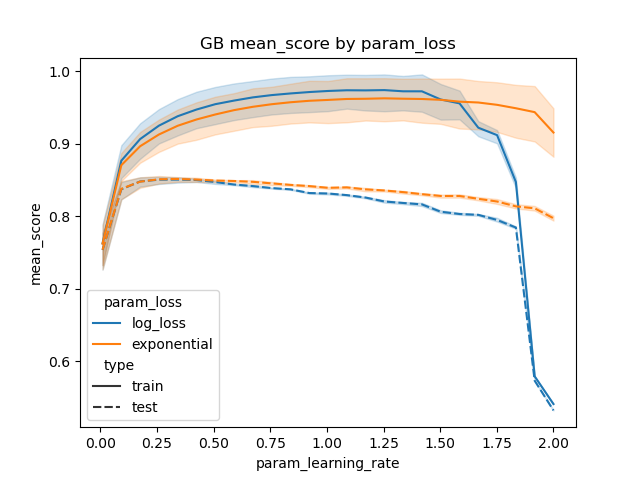
\includegraphics[width=.95\textwidth]{../results/gb/param_loss_mean_score_param_learning_rate.png}
    \caption{Performance Grouped by learning Rate}
    \end{subfigure}%
  \begin{subfigure}{.5\textwidth}
    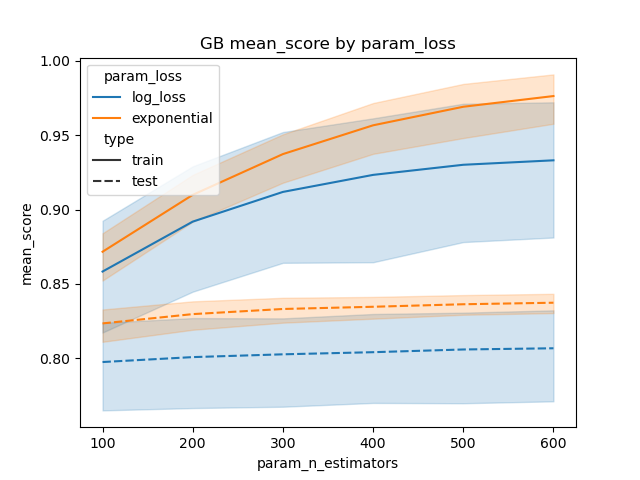
\includegraphics[width=.95\textwidth]{../results/gb/param_loss_mean_score_param_n_estimators.png}
    \caption{Performance Grouped by Estimators}
  \end{subfigure}
  \caption{GB Performance}
  \label{figure1}
\end{figure}
\subsection{KNN}
For the KNN classifier, I gridsearched combinations in the Distance metric and the number of neighbors. 
The number of neighbors varied from 1 to 100, and the Distance metric could be 'uniform','distance' or a 
custom Radial Basis function. I did not also loop over the possible parameters for the rbf, since including it was a
bonus in it's own right. The resulting performances is shown in Figure \ref{figure1}.


\begin{figure}
  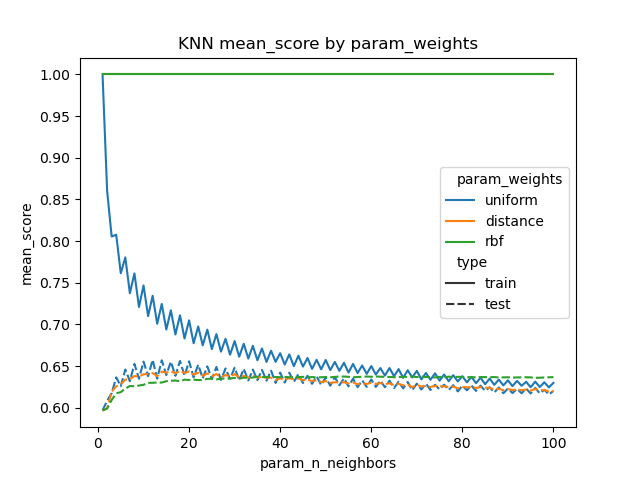
\includegraphics[width=.95\textwidth]{../results/knn/param_weights_mean_score_param_n_neighbors.png}
  \caption{KNN Performance Grouped by Metric}
  \label{figure2}
\end{figure}

This plot shows that the distance and radial basis functions drastically increased training accuracy to be 100\% at all 
values, but did not have a dramatic impact on test performance. This leads me to the conclusion that the non-uniform 
weighting increases the complexity of our models which opens us up to overfitting.

Interestingly, the uniform parameter showed a stairstep behavior where the even number neighbor counts outperformed
the next and previous odd-number amount of neighbors. That's something that caught me by surprise, and I can't quite explain.
This behavior worked in the favor of the uniform distribution, allowing it to peak higher than the other weights. So, 
the best parameter for the weight was the uniform option, which gave better test scores and showed less overfitting.

The best parameter for n\_neighbors was less intersting. We can see that it peaks pretty early in the low 10s, with 
the best parameter being achieved at n\_neighbors = 12, which gave us our final results shown in \ref{table1}.

The best KNN model generalized well, with the accuracy on the test group being quite close to it's average test performance on the 
validation splits during training. It did perform noticeably higher on the training set, but not to a degree which would 
be indicative of oppressive over-fitting. All in all, I'd say the KNN model performed quite well.


\subsection{}

\end{document}